\chapter{Wat is elektriciteit?}

Eerst gaan we bekijken wat elektriciteit nou eigenlijk is. Hoe kan het toch dat, wanneer je wat stukjes metaal tegen elkaar houdt, er een lampje kan gaan branden? \\

Om die vraag te beantwoorden, moeten we eerst een stukje natuurkunde kennen. Alles om ons heen bestaat uit kleine deeltjes die we atomen noemen. Laten we eerst zorgen dat we weten hoe een atoom precies in elkaar zit. 

\section{Atoom}
Elk atoom heeft een kern, met daar omheen een schil van elektronen. In de kern van een atoom zitten protonen en neutronen. Het aantal in de kern aanwezige protonen bepaalt welk element het is. Alle elementen die bekend zijn staan in het \href{https://nl.wikipedia.org/wiki/Periodiek_systeem}{periodiek systeem}. Koolstof, een in de natuur veel voorkomend element, heeft bijvoorbeeld 6 protonen in de kern. In Figuur \ref{fig:modelKoolstofatoom} is het model van een koolstofatoom te zien.

\begin{figure}[h!]	
	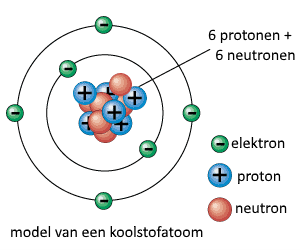
\includegraphics[scale=0.7]{./img/model_koolstofatoom.png}
	\centering
	\caption[caption]{Model van koolstofatoom \\\hspace{\textwidth} bron: https://www.sciencespace.nl/vraagbaak/5622}
	\label{fig:modelKoolstofatoom}
\end{figure}

\subsection{Elektrische lading}
In het atoom draait het om de balans in elektrische lading. De protonen hebben een positieve lading en de neutronen daarentegen hebben geen lading. Om het evenwicht te bewaren, moet er iets zijn met negatieve lading. Waarschijnlijk raad je het al: hier zorgen de elektronen voor. Door het verschil in positieve en negatieve lading zijn deze tot elkaar aangetrokken. De eenheid van deze elektrische lading is \href{https://nl.wikipedia.org/wiki/Coulomb_(eenheid)}{Coulomb}. De lading per elektron is $-1.602 \cdot 10^{-19}$ en per proton $+1.602 \cdot 10^{-19}$ Coulomb, een ontzettend klein getal. Deze heffen elkaar dus precies op. Oké, gaaf, maar wat heeft dit met elektriciteit te maken? 

\subsection{Elektrische stroom}
We weten nu dat elektronen als een schil om de atoomkern heen zitten. Nu komt het zelden voor dat een atoom in zijn eentje rondzweeft. Vaak zitten er meerdere atomen tegen elkaar, waardoor deze schillen van elektronen ook tegen elkaar aan zitten. Dan kan het voorkomen dat de elektronen van het ene atoom overspringen naar het andere atoom. De elektronen zitten namelijk niet vast maar kunnen bewegen, zo lang de elektrische lading per atoom maar in balans blijft. Stel je nu eens voor dat er 10 atomen in een kring zitten. Deze atomen geven allemaal, per seconde, één elektron naar rechts door. De elektronen bewegen dan met een snelheid van 1 per seconde in de rechter richting door de kring. Nu spreken we van een elektrische stroom, met de eenheid \href{https://en.wikipedia.org/wiki/Ampere}{Ampère}. \\

Met het aantal Ampère wordt uitgedrukt hoeveel Coulomb per seconde stroomt. Voor een stroom van 1 Ampère hebben we 1 Coulomb aan lading per seconde nodig. In formulevorm is dit:

\begin{equation}
	I = \frac{Q}{t}
\end{equation}

Waar I de elektrische stroom in Ampère, Q de elektrische lading in Coulomb en t de tijd in seconden zijn. Dus, omgeschreven naar \href{https://nl.wikipedia.org/wiki/Natuurkundige_grootheden_en_eenheden}{eenheden}, krijg je:

\begin{equation}
	\text{Ampère} = \frac{\text{Coulomb}}{\text{seconde}}
\end{equation}

Stel, je wil een stroom van 1 Ampère laten lopen door een draad. Je weet dat elke elektron een lading van $-1.602 \cdot 10^{-19}$ Coulomb heeft. Ook weet je dat, om een stroom van 1 Ampère te laten lopen, er 1 Coulomb per seconde nodig is. Voor 1 Coulomb aan lading zijn $6,242,197,253,433,208,489$ elektronen nodig. Tel jij ze? Misschien is het je al opgevallen dat er eigenlijk een negatief aantal elektronen nodig zijn om aan die 1 Coulomb te komen. Waarom dit is komen we later op terug. \\

Je bent nu bekend met elektrische lading en stroom, maar hoe kan het toch dat die elektronen gaan stromen? Gebeurt dat zomaar, of moet hier iets voor gebeuren? Goede vragen!

\subsection{Elektrische Spanning}
Elektronen gaan natuurlijk niet zomaar stromen. Als jij op de fiets zit, gaat die ook niet zomaar rijden. Daarvoor moet je een kracht uitoefenen op je trappers. Met elektronen is het net zo; je moet er een kracht op uitoefenen om ze te laten stromen. Deze kracht noemen we \href{https://nl.wikipedia.org/wiki/Elektrische_spanning}{elektrische spanning}, uitgedrukt in de eenheid \href{https://nl.wikipedia.org/wiki/Volt_(eenheid)}{volt}. Spanning is relatief, wat betekent dat het verschil in spanning tussen twee plekken van belang is, en niet de absolute waarde. Je kunt dit vergelijken met \href{https://nl.wikipedia.org/wiki/Touwtrekken}{touwtrekken}. Als beide teams precies even hard aan het touw trekken, dan blijft het touw alsnog in het midden. Het verschil in spanning zorgt voor een kracht op de elektronen, waardoor deze als het ware van het ene atoom naar het andere worden geduwd.

\subsection{Elektrische weerstand}
Dan is er nog zoiets als \href{https://nl.wikipedia.org/wiki/Elektrische_weerstand_(eigenschap)}{elektrische weerstand}, uitgedrukt in \href{https://nl.wikipedia.org/wiki/Ohm_(eenheid)}{Ohm} (symbool Ω). Je hebt net geleerd dat het kracht kost om elektronen te laten stromen. Hoeveel kracht dit kost, is afhankelijk van de weerstand van het materiaal waar de elektronen door stromen. De weerstand van een materiaal is afhankelijk van het element waar het van is gemaakt. Bij sommige elementen geven de atomen hun elektronen minder graag door aan hun buren, waar anderen dit juist makkelijker doen. Wanneer het weinig kracht (lage spanning) kost om een elektron door te geven, spreken we van een lage weerstand. Kost het veel kracht (hoge spanning), dan heeft het element een hoge weerstand. \\

Wanneer een element een hoge weerstand heeft noemen we dit een goede isolator, wanneer het een lage weerstand heeft een geleider. Rubber isoleert bijvoorbeeld erg goed, waar metaal juist heel goed geleid. Kijk eens naar de draden van een project dat je gemaakt hebt. Valt er iets op? \\

Om even veel elektronen te laten stromen door iets met een hogere weerstand, heb je dus een hogere spanning nodig. Maar hoeveel hoger moet die zijn? Hier komt de \href{https://nl.wikipedia.org/wiki/Wet_van_Ohm}{wet van Ohm} om de hoek kijken. Deze wet beschrijft het verband tussen spanning, stroom en weerstand als volgt:

\begin{equation}
	U = I \cdot R
\end{equation}

Met spanning U in Volt, stroom I in Ampère en weerstand R in Ohm. Omgeschreven naar deze eenheden krijg je dus:

\begin{equation}
	\text{Volt} = \text{Ampère} \cdot \text{Ohm}
	\label{eq:ohmslaw_volt_unknown}
\end{equation}

Het is ook mogelijk om de stroom te berekenen:

\begin{equation}
	\text{Ampère} = \frac{\text{Volt}}{\text{Ohm}}
	\label{eq:ohmslaw_ampere_unknown}
\end{equation}

Of de weerstand:

\begin{equation}
	\text{Ohm} = \frac{\text{Volt}}{\text{Ampère}}	
	\label{eq:ohmslaw_ohm_unknown}
\end{equation}

Zoals je ziet zijn er maar twee van de drie (spanning, weerstand, stroom) nodig om ze alle drie te weten te komen. Voor een extra geheugensteuntje, zie Figuur \ref{fig:ohmslawtriangle}. 

\begin{figure}[H]
	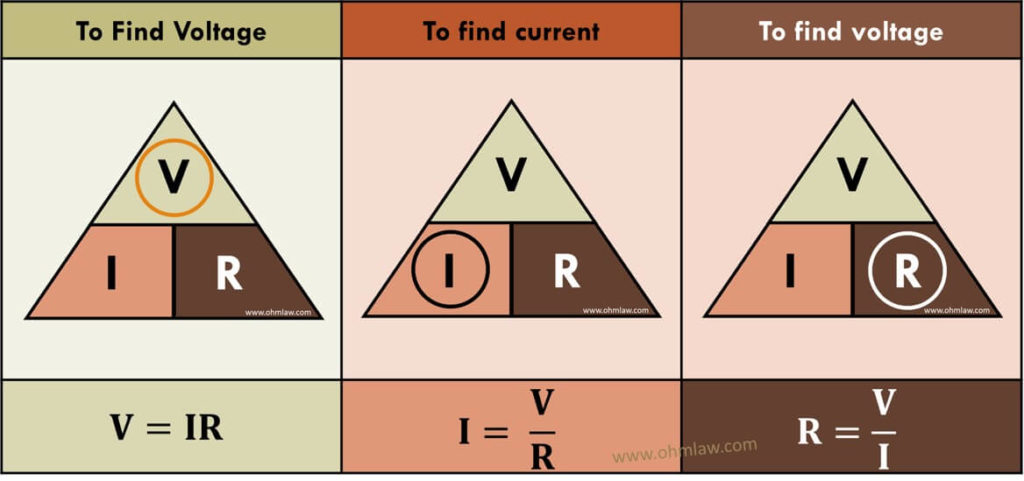
\includegraphics[scale=0.3]{./img/ohms_law_triangle.jpg}
	\centering 
	\caption[caption]{Wet van Ohm geheugensteuntje \\\hspace{\textwidth} bron: https://ohmlaw.com/ohms-law-triangle/}
	\label{fig:ohmslawtriangle}
\end{figure}

Zo, nu weet je wat elektrische lading, spanning, stroom en weerstand zijn en ken je de wet van Ohm. Maar waar komt die spanning of stroom vandaan? Dat komt nu aan bod.

\section{Elektrisch netwerk}
\href{https://nl.wikipedia.org/wiki/Elektrisch_netwerk}{Elektrische netwerken} bestaan uit twee delen: een bron en een verbruiker. Bijvoorbeeld, een batterij die de elektriciteit levert, en een lampje dat het verbruikt. Eerst gaan we ons richten op de bron van de elektriciteit, en hoe we daarmee kunnen rekenen. \\

In Figuur \ref{fig:elektrischnetwerk} zie je een schema van een simpel elektrisch netwerk. Er is een spanningsbron (aangeduid met V) en een weerstand (aangeduid met R) te zien. Ook is de richting van de stroom aangegeven met i.
\begin{figure}[h!]
	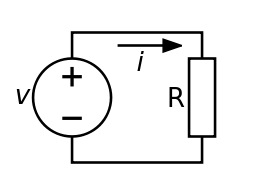
\includegraphics[scale=0.5]{./img/elektrisch_netwerk.png}
	\centering
	\caption{Elektrisch netwerk}
	\label{fig:elektrischnetwerk}
\end{figure}

\textbf{Rekenvoorbeelden} \\
1) De spanningsbron is 9 Volt en de weerstand is 10 Ohm. Hoeveel Ampère is stroom i? 
Hiervoor kan je Vergelijking \ref{eq:ohmslaw_ampere_unknown} gebruiken, waarbij je de spanning door de weerstand deelt. 

\begin{equation}
	i = \frac{9V}{10\Omega} = 0.9A
\end{equation}

2) De stroom is $2A$ en de weerstand $24 \Omega$, wat is spanning $V$? Denk terug aan Vergelijking \ref{eq:ohmslaw_volt_unknown} en bereken het als volgt:
\begin{equation}
	V = 2A \cdot 24 \Omega = 48V
\end{equation}

3) De spanning is 1.5V en de stroom is 0.75A, wat is weerstand $\Omega$? Zie Vergelijking \ref{eq:ohmslaw_ohm_unknown} en bereken als volgt
\begin{equation}
	\Omega = \frac{1.5V}{0.75A} = 2 \Omega
\end{equation}

\subsection{Spanning- en stroombron}
Doorgaans maken we onderscheid tussen twee bronnen: een spanningsbron en een stroombron. De schematische weergaves zijn weergeven in Figuur \ref{fig:spanningsbron} en Figuur \ref{fig:stroombron}.

\begin{figure}[H]
	\begin{minipage}{0.45\textwidth}
		\centering
		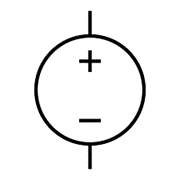
\includegraphics[scale=0.5]{./img/spanningsbron.png}
		\caption{Spanningsbron}
		\label{fig:spanningsbron}
	\end{minipage}
	\hfill
	\begin{minipage}{0.45\textwidth}
		\centering
		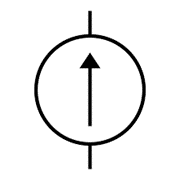
\includegraphics[scale=0.5]{./img/stroombron.png}
		\caption{Stroombron}
		\label{fig:stroombron}
	\end{minipage}
\end{figure}


Het verschil tussen deze twee is dat een spanningsbron een vaste spanning levert, waar een stroombron een vaste stroom levert. Bij een spanningsbron gaat er natuurlijk ook gewoon stroom lopen, maar de hoeveelheid is afhankelijk van wat er aan verbonden is. Een stroombron levert ook gewoon spanning, alleen past die de spanning zo aan dat de gewenste stroom gaat lopen, afhankelijk van de verbonden weerstand. \\

Maar hoe bouw je een spannings- of stroombron? Wanneer je een batterij pakt, staat hier altijd een voltage op. Een AA-batterij levert doorgaans 1.5 volt en een blokbatterij 9 volt. Daar is je spanningsbron. Een stroombron is wat lastiger om te maken, dus dat komt later. \\

\subsection{Serie- en parallel schakelingen}
Waarschijnlijk heb je er al wel eens van gehoord, maar wat is het nou precies? Een serie- of parallel schakeling geeft aan hoe elektrische componenten, zoals weerstanden, met elkaar verbonden zijn in het elektrische netwerk.

Bij een \href{https://nl.wikipedia.org/wiki/Serieschakeling}{serieschakeling} zijn de componenten na elkaar geschakeld. Denk maar aan een ketting, het is een lange draad van componenten. \\

Een \href{https://nl.wikipedia.org/wiki/Parallelschakeling}{parallelschakeling} betekent dat de componenten allemaal naast elkaar geschakeld staan. 

\subsection{Wetten van Kirchhoff}
TODO

\section{Elektriciteit en energie}
Er wordt vaak gesproken over elektrische energie, maar wat is dat eigenlijk en hoe kan je ermee rekenen? 

\begin{itemize}
	\item energie, wat is dat (Joules)
	\item Elektrisch vermogen
	\item 
\end{itemize}

$\infty ^{\circ}$
